
\documentclass[11pt]{article} % Default font size is 12pt, it can be changed here
\usepackage{geometry} % Required to change the page size to A4
\geometry{a4paper} % Set the page size to be A4 as opposed to the default US Letter
\usepackage{graphicx} % Required for including pictures
\usepackage{hyperref}
\usepackage{array}

\usepackage{float} % Allows putting an [H] in \begin{figure} to specify the exact location of the figure
\usepackage{wrapfig} % Allows in-line images such as the example fish picture
\usepackage{lipsum} % Used for inserting dummy 'Lorem ipsum' text into the template
\linespread{1.2} % Line spacing

\graphicspath{{./Pictures/}} % Specifies the directory where pictures are stored
\usepackage{url}

% to remove coloured boxes around the links 
\hypersetup{
    colorlinks=false,
    pdfborder={0 0 0},
}
\newenvironment{myindentpar}[1]%
 {\begin{list}{}%
         {\setlength{\leftmargin}{#1}}%
         \item[]%
 }
 {\end{list}}
%----------------------------------------------------------------------------------------
\begin{document}
%----------------------------------------------------------------------------------------
\begin{titlepage}
\newcommand{\HRule}{\rule{\linewidth}{0.5mm}} % Defines a new command for the horizontal lines, change thickness here
\center % Center everything on the page

\includegraphics{urjc} \\[0.5cm] % Include logo
\textsc{\LARGE \\Universidad Rey Juan Carlos}\\[1cm] % Name of your university/college
\textsc{\Large Master in Libre Software}\\[0.5cm] % Major heading such as course name
\HRule \\[1.5cm]
{ \huge \bfseries Case Study II.}\\[0.4cm] % Title of your document
\HRule \\[1.5cm]
\begin{minipage}{0.4\textwidth}
\begin{flushleft} \large
\emph{Authors:}\\
Amal \textsc{Roumi}\\ % Your name
\end{flushleft}
\end{minipage}
%~
\begin{minipage}{0.4\textwidth}
\begin{flushright} \large
\emph{Supervisor:} \\
Gregorio  \textsc{Robles} % Supervisor's Name
\end{flushright}
\end{minipage}\\[1.5cm]
{\large \today}\\[1.8cm] % Date, change the \today to a set date if you want to be precise
\textsc CC BY-NC-SA 3.0\\[0.2cm]

\includegraphics[scale=0.5]{license} \\ % Include license
{\small http://creativecommons.org/licenses/by-nc-sa/3.0}\\
\mbox{}

\end{titlepage}

%================================================================================

\par As final work for the course of “Case Studies II” in 2012/2013 in Master of Libre software (Universidad Rey Juan Carlos), we are requested to write horizontal  report one topic we choose in each projects that have been presented in this subject,  my choice was “ License”.  
\section{Aspects of Licenses}

In any discussion of open source licensing, the first thing that becomes apparent is that there seem to be many different terminology, we will talk about them in the following lists
\\*

{\bf Free software, open source software} 
Software that granting the four freedom-rights. users are free to run, copy, distribute, study, change and improve the software.
This term was first coined by Richard Stallman, who codified it in the GNU General Public License (GPL), and who founded the Free Software Foundation\footnote{\url { http://www.fsf.org/}} . "free software" covers almost exactly the same range of software as "open source"which was coined by the Open Source Initiative\footnote{\url{http://www.opensource.org/}} .Open source software and free software typically describe the same programs, the two terms are commonly used interchangeably. And it is said that the difference between them is philosophical rather than practical and that the difference between the two terms themselves is mainly a matter of marketing rather than substance.

{\bf DFSG-compliant} 
Compliant with the Debian Free Software Guidelines (DFSG )  \footnote{\url{http://www.debian.org/social_contract}}
which is a set of guidelines that the Debian Project uses to determine whether a software license is a free software license, which in turn is used to determine whether a piece of software can be included in Debian.
  
{\bf OSI-approved} 
Approved by the Open Source Initiative. The OSI's definition of open source software is based on the Debian Free Software Guidelines,  the OSI maintains a list of all licenses it has ever approved, at \url {http://www.opensource.org/licenses/}, 

{ \bf Proprietary, closed-source}
Software distributed under exclusive legal right of the copyright holder with the intent that the licensee is given the right to use the software only under certain conditions, and restricted from other uses, such as modification, sharing, studying, redistribution

{ \bf Contributor License Agreements (CLA)}
Define the terms under which intellectual property has been contributed to a company/project and thereby allow them to defend the project should there be a legal dispute regarding the software at some future time. 
The purpose of a CLA is to
 Ensure that the guardian of a project's outputs has the necessary ownership or grants of rights over all contributions to allow them to distribute under the chosen license.
Protect community members (both developers and users) from intellectual property lawsuits if needed.
We have to mention that the license agreement does not transfer copyright ownership and does not change the contributors rights to use their own contributions for any other purpose.
%================================================================================
\section{Some common open source license.}
%------------------------------------------------

{\bf GNU General Public License (GPL)}
Written by :Richard Stallman of the Free Software Foundation (FSF) for the GNU project.
\\* 
Versions:There are three different versions of the GPL License .\\* 
The latest version was GPL v3.0 at June 2007\\* 
The (GPL) is probably one of the most commonly used licenses for open-source projects. The GPL grants and guarantees a wide range of rights to developers who work on open-source projects. Basically, it allows users to :
\begin{enumerate}
\item Copy the software
\item Distribute the software however you want.
\item Charge a fee to distribute the software.
\item Make whatever modifications to the software you want.
\end{enumerate}
%------------------------------------------------
 
{\bf BSD licenses}
 Originally created by the University of Berkeley. BSD licenses represent a family of permissive free software licenses that have fewer restrictions on distribution compared to other free software licenses.
 Among different versions of the license two versions : the New BSD License/Modified BSD License, and the Simplified BSD License/FreeBSD License. Both have been verified as GPL-compatible free software licenses, and have been accepted as open source licenses by the Open Source Initiative \\* 
%------------------------------------------------

{\bf MIT License}
Written by : Massachusetts Institute of Technology (MIT)\\* 
The latest version was at 1988\\* 
It is shortest and probably broadest of all the popular open-source licenses. Its terms are very loose and more permissive than most other licenses. The MIT License is the least restrictive license out there. It basically says that anyone can do whatever they want with the licensed material, as long as it’s accompanied by the license.\\* 
%------------------------------------------------

{\bf  Apache License}
Written by : Apache Software Foundation (ASF) \\* 
Versions:There are three different versions of the Apache License .\\* 
The latest version was Apache v2.0 at 2004\\* 
The Apache License, Version 2.0, grants a number of rights to users. These rights can be applied to both copyrights and patents. 
Because some licenses can be applied only to copyrights and not patents, this flexibility would be an obvious factor in a patent developer’s choice of license
Here are some on what the Apache License allows:\\* 
Rights are perpetual, non-exclusive ,, worldwide, irrevocable.\\* 
Rights are granted for no fee or royalty.\\* 
%------------------------------------------------

{\bf The Mozilla Public License (MPL)}\\* 
Written by : Mozilla Foundation .\\* 
Versions:There are three different versions of the MPL License .\\* 
The latest version was MPL v2.0 at 2012\\* 
It is characterized as a hybridization of the modified BSD license and GNU General Public License (GPL) that seeks to balance the concerns of proprietary and open source developers.
%================================================================================

\section{Briefs about each project and their licenses.}
%------------------------------------------------

\subsection{Apache} % Sub-section
\url {http://www.apache.org} 
The Apache Software Foundation (ASF) non-profit corporation, provides organizational, legal, and financial support, founded in 1999.\\*
Among the ASF's objectives are: 
\begin{enumerate}
\item  to provide legal protection to volunteers working on Apache projects.
\item to prevent the Apache brand name from being used by other organizations without permission.
\end{enumerate}
The Apache Software Foundation is a decentralized community of developers. The software they produce is distributed under the terms of the Apache License and is therefore free and open source software (FOSS).\\*
{\bf Licensing}
All software produced by The Apache Software Foundation or any of its projects  is licensed under  Apache License , the current version is 2.0 \footnote{\url{http://www.apache.org/licenses/LICENSE-2.0}} the Apache License is compatible with the GPL license.\\*  
The ASF desires that all contributions of code, or documentation to the Apache projects sign, and submit the Contributor License Agreement (CLA)
%------------------------------------------------

\subsection{WebKit} % Sub-section
Website \url {http://www.webkit.org}
Webkit is an open source web browser engine that was original author by KDE and developed  by Apple , Google ,adobe.. \\*
Currently powers browsers such as Google Chrome, Apple Safari, the default IOS browser, and the default Android browser, opera,blackberry \\*
WebKit's HTML and JavaScript code originally began as a fork of the KHTML and KJS libraries from KDE, and has now been further developed by individuals from KDE, Apple, Google, Nokia, Bitstream, RIM, Igalia, and others. OS X, Windows, GNU/Linux, and some other Unix-like operating systems are supported by the project.\\*
{\bf Licensing}
WebKit's WebCore and JavaScriptCore components are available under the GNU Lesser General Public License  \footnote{\url{http://www.gnu.org/copyleft/lesser.html}} , and the rest of WebKit is available under a BSDl licenses \footnote{\url{http://www.webkit.org/coding/bsd-license.html }}

%------------------------------------------------
\subsection{Plan 9 from Bell Labs} % Sub-section
Website: \url {http://plan9.bell-labs.com/plan9/index.html}
A free software distributed operating system. by ATT Bell Laboratories , the research and development subsidiary of the French-owned Alcatel-Lucent in Berkeley Heights, New Jersey, United States.Plan9.Starting in the late 1980s. It was designed and developed by the inventors of the UNIX operating system created at Bell Labs and is an evolution of UNIX design concepts:
\begin{itemize}
\item All objects are either files or file systems
\item Communication is over a network.
\item Private namespaces allow their owners to access local and remote processes transparently
\end{itemize}
The name Plan 9 from Bell Labs is a reference to the science fiction movie” Plan 9 from Outer Space”. Also, the Plan 9 Bunny, is presumably a reference to Wood's film Glen or Glenda.\\*
To reduce the number of custom APIs and system calls, Plan 9 use the 9P . The protocol is used to refer to and communicate with processes, programs, and data, including both the user interface and the network.\\*
{\bf Licensing}
Plan 9 has had four major releases over its lifetime here they are and their licensing:
\begin{itemize}
\item The first edition was released in 1992 made available only for use by universities.
\item The second edition was released in 1995 in book-and-CD made available to the general public with fees for the distribution, which included a license to use the software throughout the organization.
\item For the third edition, was released in June 2000, Lucent agreed to release Plan 9 for free via the Internet, under a new license, the Plan 9 License.
\item The fourth edition (the current one)was release, in 2002 is made available under the Lucent Public License version 1.02.\footnote {\url{http://opensource.org/licenses/lucent1.02.php}} Adopted to address shortcomings in the Plan 9 License, the Lucent Public License 1.02 is identical the IBM Public License 1.0 \footnote {\url{http://opensource.org/licenses/ibmpl.php}} except that it does not require source code to be distributed with derived works; it is non-viral.
\end{itemize}
The full source code is freely available under Lucent Public License 1.02 . it is considered DFSG compatible and approved by FSF and OSI. However, it is incompatible with the GNU General Public License.
%------------------------------------------------
\subsection{GMozilla - Mozilla Hispano Communities / Firefox OS} % Sub-section
Website Mozilla \url {http://www.mozilla.org/en-US/} \\*
Website Firefox OS  \url {http://www.mozilla.org/en-US/firefox/partners/}\\*
Mozilla Foundation is anon-profit organization that exists to support the open source Mozilla project.Was founded by the Netscape-affiliated Mozilla Organization in July 2003, the organization controls Mozilla trademarks and copyrights. \\*
The Mozilla Foundation describes itself as "a non-profit organization that promotes openness, innovation and participation on the Internet ”  
Mozilla is a free software community uses, develops, spreads and supports Mozilla products  like Firefox browser ,Firefox Mobile, the Firefox OS mobile operating system, the bug tracking system Bugzilla and the free email application Thunderbird .
The community is supported by the Mozilla Foundation.\\*
Firefox OS 
Is a linux-based open source operating system for smart phone and table computers. 
It is designed to allow HTML5 applications to communicate directly with the device's hardware using JavaScript. It has been demonstrated on Android-compatible smartphones, and the Raspberry Pi.
The first smartphones running Firefox OS should be released 2013 .\\
%------------------------------------------------
{\bf Licensing}
All Mozilla software is open source and free software under Mozilla Public License(MPL)
{\it summary of the Mozilla license policy:}
\begin{itemize}
\item New files in, or modifications to, an existing, consistently-licensed area of code should be under the same license as the existing code.
\item New projects should be under the MPL 2.0 or Apache 2.0 
\end{itemize}
\centerline{ The following flowchart provides a summary of Mozilla Foundation License Policy} 
\centerline{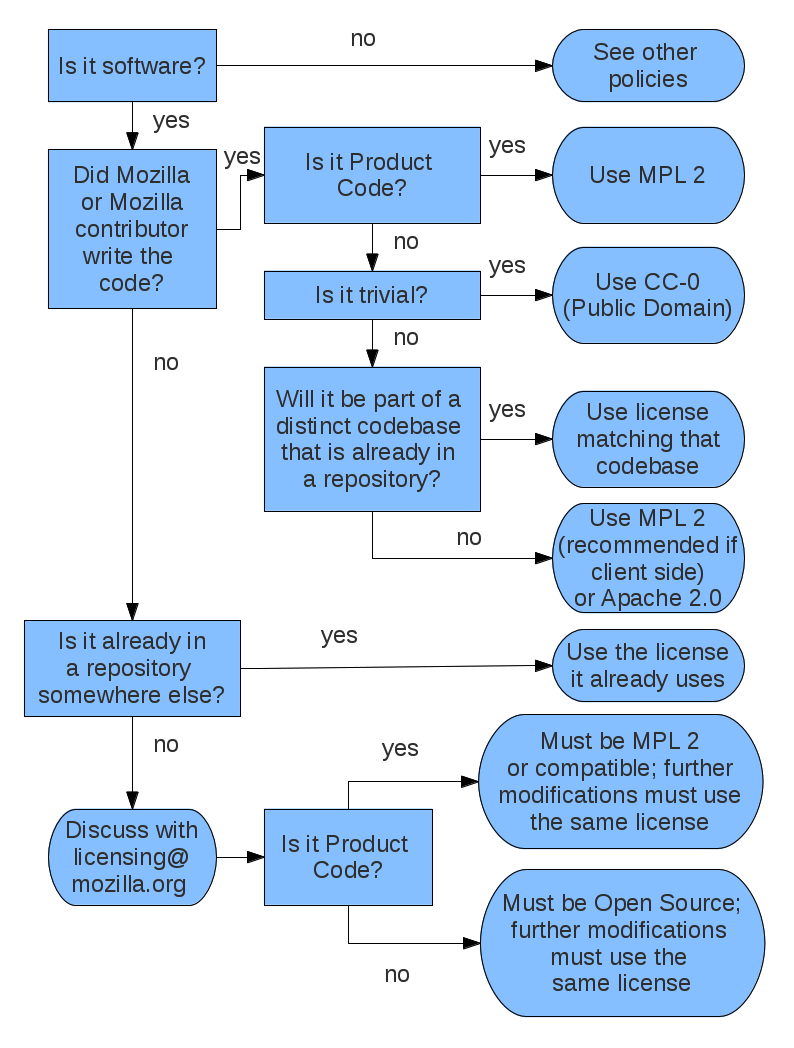
\includegraphics[scale=0.3]{chart}}
\centerline \small    source : \url {http://www.mozilla.org/MPL/license-policy-flowchart.png}
%------------------------------------------------
\subsection{GNU and GNU-es} % Sub-section
Website:\url{ http://www.gnu.org}\\*
The GNU Project was launched in 1984  by Richard Stallman to develop the GNU system. The name “GNU” is a recursive acronym for “GNU's Not Unix!”. Its aim is to give computer users the four freedom “run the software share it study it and modify it “\\*
{\bf licensing}
 the GNU General Public License (GNU GPL) used by most GNU programs,but some times use  other free software licenses that are only compatible with the GNU GPL for GNU software 
\footnote {\url {http://www.gnu.org/licenses/license-list.html\#SoftwareLicenses}}

\centerline{ The  following diagram show the license that are compatible with the GPL v3} 
\centerline{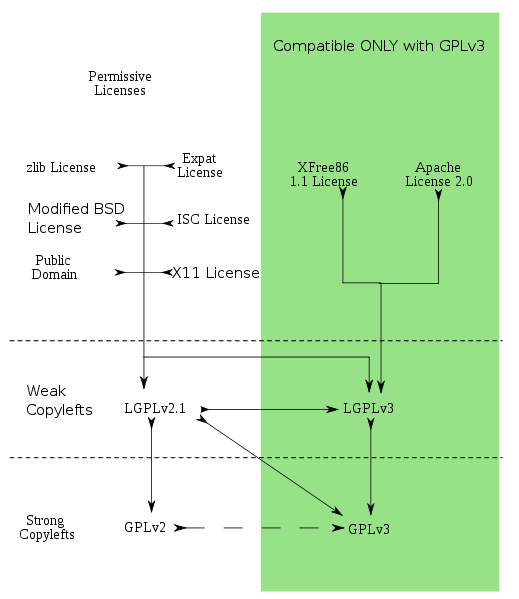
\includegraphics[scale=0.4]{gplv3-compatibility}}
\centerline \small  source \url {http://upload.wikimedia.org/wikipedia/en/5/52/Quick-guide-gplv3-compatibility.png}
%------------------------------------------------
\subsection{The Document Foundation} % Sub-section
Website \url {http://www.documentfoundation.org}\\*
The Document Foundation is a German foundation created by members of OpenOffice.org Community over fears that Oracle Corporation, after acquiring Sun Microsystems, would discontinue developing OpenOffice.org  which they were developing it in ten years .\\*
The Document Foundation created LibreOffice as an open source software under the GNU Lesser General Public License (LGPLv3).
%------------------------------------------------
\subsection{Liferay} % Sub-section
Website \url {http://www.liferay.com}\\
Liferay Portal is a free and open source enterprise portal  created in 2000 . that provides free documentation and paid professional service to users of its software. \\*
{\bf licensing}
Liferay Business Model is  dual-License . It has been under the MIT license for ten years ,but after version 6 Liferay Portal distributed under the Lesser GNU Public License (LGPL) v2.1 which provide the best benefits of the MIT license and the best protection against MIT’s limitations and under commercial licenses  (EE) \footnote {\url{http://www.liferay.com/products/liferay-portal/ee/faq}}
%------------------------------------------------
\subsection{Free Software in Public Administrations} % Sub-section
Zaragoza  aim to be  the city of knowledge\footnote {\url{http://www.zaragoza.es/ciudad/conocimiento/conocimiento.htm}} 
Zaragoza Migration Plan to free software was successful they shift from closed software to open software in three phases :
\begin{itemize}
\item Desktop Applications on Windows XP OS : Switch the application to free software like  Browser Firefox, Microsoft Outlook to Thunderbird, Media Player to Reproductor multimedia VLC
\item Office applications: Microsoft Office 97 Switch to OpenOffice.
\item  Platform : Migration of Windows XP operating system to SUSE Linux Enterprise Desktop OS AZLinux.
\end{itemize}
In order to execute this plan they need to :
\begin{itemize}
\item  Hardware and Software.
\item Technical Training.
\item Training plans necessary for municipal staff.
\end{itemize}

%------------------------------------------------
\subsection{KDE} % Sub-section

Website:\url {http://www.kde.org}\\
KDE is a Windowing Manager and Graphical User Interface , producing an integrated set of cross-platform applications designed to run on GNU/Linux, FreeBSD, Solaris, Microsoft Windows, and OS X systems.\\*
The KDE project serves as an umbrella project for many standalone applications and smaller projects that are based on KDE technology. These include Calligra Suite, digiKam, Rekonq, K3b, and many others.
All of the software that KDE produces is a Free and Open Source Software \\

{L\bf icensing} \\*
KDE, lies a graphical toolkit and fully featured programming language called Qt.

The KDE Free Qt foundation was created in 1998 under liberal BSD license which guarantees that Qt " which was dual-licensed under the free and open source Q Public License (QPL) \footnote {\url{http://opensource.org/licenses/QPL-1.0}}  and a commercial license for proprietary software developers" would fall under a variant of BSD license should Trolltech cease to exist or no free version of Qt be released during period of time.
 In 2000 Trolltech made the Unix version of the Qt libraries available under the GNU General Public License (GPL), in addition to the QPL.
After Qt 4.5, proprietary applications can legally use the open source Qt version.
Because Qt available under the LGPL version 2.1.\\*
 KDE Platform consists of the libraries and services needed to run KDE applications. The libraries must be licensed under one of the LGPL, BSD license, MIT License and X11 license.\\*
KDE's adoption of the Fiduciary Licence Agreement (FLA) The FLA is a copyright assignment that allows Free Software projects to assign their copyright to single organisation or person. This enables projects to ensure their legal maintainability, including important issues such as preserving the ability to re-license and certainty to have sufficient rights to enforce licences in court.

%------------------------------------------------
\subsection{GNOME} % Sub-section

Website:\url {http://www.gnome.org}\\*
GNOME is a user-friendly and completely free desktop environment and graphical user interface that runs on top of a computer operating system . developed by both volunteers and paid contributors, the largest corporate contributor being Red Hat. \\*
GNOME is part of the GNU Project and can be used with various Unix-like operating systems.
\\* 
{\bf Licensing}
GNOME is licensed under the LGPL for its libraries, and the GNU General public licenses (GPL) for its applications.

%------------------------------------------------
\subsection{QA in Thunderbird} % Sub-section

Website \url {http://www.mozilla.org/en-US/thunderbird/}\\*
Mozilla Thunderbird is a free, open source, cross-platform email, news and chat client developed by the Mozilla Foundation \\*
In, 2012, Mozilla announced that they had come to the conclusion that continued innovation in Thunderbird is not a priority for Mozilla’s product efforts.
 The new development model is based on Mozilla offering only "Extended Support Releases"(ESR), which deliver security and maintenance updates, while allowing community to take over the development of new features.
Thunderbird QA is run by one Mozilla employee “ Ludovic Hirlimann” his role is about the “test plan”. This is the plan that documents the strategy that will be used to verify and ensure that a product meets its design specifications and other requirements.\\*
{\bf Licensing}
Mozilla Thunderbird  licensed under the MPL 

%------------------------------------------------
\subsection{Canonical} % Sub-section
Website \url {http://www.canonical.com}
\\* Canonical is privately held computer software company founded by Mark Shuttleworth to market commercial support and related services for Ubuntu and related projects , Canonical release first Ubuntu on 2004  under GNU GPLlicenses and other free software licenses.\\*
Canonical Ltd. has created and continues to back several projects. Principally these are free/open-source software (FOSS) or tools designed to improve collaboration between free software developers and contributors.\\*
Canonical working on a number of open-source projects including:Launchpad,Bazaar
The Canonical uses  Contributor License Agreement  for all contributions to many projects established by Canonical.\\
Some of the rojects requiring contributors to sign this agreement are Launchpad, OpenStack,Ubuntu One and more 

%------------------------------------------------
\subsection{OSOR} % Sub-section
Website \url {http://joinup.ec.europa.eu/page/osor.eu}\\*
OSOR is an acronym standing for “Open Source Observatory and Repository” for European public administrations
Project financed by E.C. and managed by IDABC \footnote {stands for:
Interoperable Delivery of pan-European eGovernment Services to Public Administrations,
Businesses and Citizens}
Supported by the Member State administrations.\\*

 OSOR.eu platform, and in particular the OSOR.eu Repository and the OSOR.eu Forge are aimed to support and encourage use of OSS or FLOSS for Free, Libre and Open Source Software that are of particular use for public administrations in Europe. \\
In December 2011, Osor.eu was migrated to a new collaborative platform: Joinup.

{\bf OSOR Main Services \footnote {\url{http://joinup.ec.europa.eu/sites/default/files/OSOR_dissemination-Tampere-2008.pdf}}}

\begin{enumerate}
   \item Information platform
  \begin{enumerate}
		\item Website delivering news around OSS
		 \item -  Providing guidance on legal, technical, organizational issues around OSS and collaboration.
	\end {enumerate}
   \item Registry and Repository
	\begin{enumerate}
		\item -  Facilities for download and uploading and search and retrieval of public sector software .
		\item Providing visibility for and connect to other European collaboration platforms.
	\end {enumerate}
   \item  Platform for collaboration 
	\begin{enumerate}
		\item - Supporting collaborative cross-border projects (hosting communities)
	\end {enumerate}
  \item EUPL: European Union Public License
	\begin{enumerate}
		\item Legal instrument for the EC and the EU public sector
	\end{enumerate}
\end {enumerate}
\newpage
%====================================================================
\section{Conclusions}
This paper we talked about the  licenses in open source project ,  between lenient, like the BSD, and strict, like the GNU GPL and MPL . 
and about the community around them .\\* 
we also discussed  some topics that is not a project or a company  for example "  Free Software in Public Administrations" .It is  a good example for migration in Zaragoza city to the open source world , and in my personal view it is  good  model  if we can  copy the experience to the other cities after looking at the advantages and disadvantages of their migration .
In the following we have some comparative between the projects in the matter of license from  full rights to no rights.
but we can see that most of them are under GPL or LGPL which is the most common license in free software.
\centerline{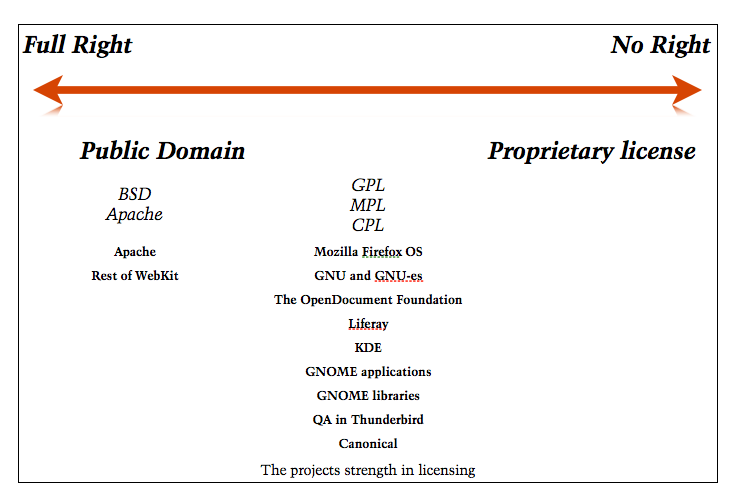
\includegraphics[scale=0.6]{Theprojects}}
\\
In the nest table 1  Open Source licenses comparison table between the  most common license  when releasing new project
%----------------------------------------------------------------------------------------
\begin{table}[ht]
\caption{Comparison between the license in derived work}
\centering
\begin{tabular}{c  m{3cm}  m{4cm} m{3cm}}
\hline\hline

License name & Different name in  DW & DW remains OS & Change license type for DW \\ [3ex]

\hline
Apache License 2.0&Yes&No&Yes \\
(GPLv2)& yes but should mark changes & yes only if published& yes for compatible \\
LGPL&Yes& same as in GPL, but can link compiled libraries & yes for compatible \\
(MPL)1.1 & Yes & No & No \\
BSD License & Yes & No & Yes \\ [1ex]
\hline\hline
\end{tabular}
\label{table:nonlin}
\end{table}

%----------------------------------------------------------------------------------------
%	 References
%----------------------------------------------------------------------------------------
\newpage

\centerline \small {* DW for derived work}
\newpage 
{\bf References}\\*
	\begin {enumerate}
	\item \url {http://www.oss-watch.ac.uk/resources/cla}
	\item \url {http://www.liferay.com/web/bryan.cheung/blog/-/blogs/liferay-adopting-the-lgpl-license}
	\item \url {http://www.zaragoza.es/ciudad/conocimiento/conocimiento.htm}
	\item\url {http://joinup.ec.europa.eu}
	\end {enumerate}
\newpage

%  table of contents
%----------------------------------------------------------------------------------------
\tableofcontents

\end{document}
